\documentclass[12pt,a4paper]{report}

%adjust your page margins here
\usepackage[top=0.70in, bottom=0.70in, left=0.8in,right=0.80in]{geometry} % setting the page alignment with this package
\usepackage[pdftex]{graphicx} %for embedding images
\usepackage[%dvips, % commented for pdflatex
bookmarks,  colorlinks=false]{hyperref} %for creating links in the pdf version and other additional pdf attributes, no effect on the printed document
\hypersetup{%
    pdfborder = {0 0 0}
}
\usepackage[final]{pdfpages} %for embedding another pdf, remove if not required
\usepackage{float} %used for figure placement with H as a parameter
\usepackage{hyperref}
\usepackage{pslatex} % for times new roman, old package, but works
\usepackage{array} % for making text bold in table
\usepackage{setspace}
\usepackage{float}
\usepackage{enumerate}
\usepackage{longtable}

\usepackage[font=small,labelfont=bf]{caption}
\def\figurename{\textbf{Figure }}

\usepackage{listings}
\usepackage{color}

\definecolor{dkgreen}{rgb}{0,0.6,0}
\definecolor{gray}{rgb}{0.5,0.5,0.5}
\definecolor{mauve}{rgb}{0.58,0,0.82}
 
\lstset{ %
  language=Java,                % the language of the code
  basicstyle=\footnotesize,           % the size of the fonts that are used for the code
  numbers=left,                   % where to put the line-numbers
  numberstyle=\tiny\color{gray},  % the style that is used for the line-numbers
  stepnumber=1,                   % each line is numbered
  numbersep=5pt,                  % how far the line-numbers are from the code
  backgroundcolor=\color{white},      % choose the background color. You must add \usepackage{color}
  showspaces=false,               % show spaces adding particular underscores
  showstringspaces=false,         % underline spaces within strings
  showtabs=false,                 % show tabs within strings adding particular underscores
  frame=single,                   % adds a frame around the code
  rulecolor=\color{black},        % if not set, the frame-color may be changed on line-breaks within not-black text (e.g. commens (green here))
  tabsize=2,                      % sets default tabsize to 2 spaces
  captionpos=b,                   % sets the caption-position to bottom
  breaklines=true,                % sets automatic line breaking
  breakatwhitespace=false,        % sets if automatic breaks should only happen at whitespace
  title=\lstname,                   % show the filename of files included with \lstinputlisting;
                                  % also try caption instead of title
  keywordstyle=\color{blue},          % keyword style
  commentstyle=\color{dkgreen},       % comment style
  stringstyle=\color{mauve},         % string literal style
  escapeinside={\%*}{*)},            % if you want to add a comment within your code
  morekeywords={*,...}               % if you want to add more keywords to the set
}

%For the header and footer
\usepackage{fancyhdr}
\fancypagestyle{plain}{%
\fancyfoot[L]{\emph{IIIT Kalyani}} % except the center
\fancyfoot[R]{\thepage}
\renewcommand{\headrulewidth}{0.4pt}
\renewcommand{\footrulewidth}{0.4pt}
}

\pagestyle{fancy}

\rhead{\emph{Fault Attack on RoadRunneR}}

\fancyfoot[LO,LE]{\emph{IIIT Kalyani}}
\cfoot{}
\fancyfoot[RO, RE]{\thepage}
\renewcommand{\headrulewidth}{0.4pt}
\renewcommand{\footrulewidth}{0.4pt}
%For the header and footer Over

%Page Border
\usepackage{pgf}
\usepackage{pgfpages}

\pgfpagesdeclarelayout{boxed}
{
  \edef\pgfpageoptionborder{0pt}
}
{
  \pgfpagesphysicalpageoptions
  {%
    logical pages=1,%
  }
  \pgfpageslogicalpageoptions{1}
  {
    border code=\pgfsetlinewidth{2pt}\pgfstroke,%
    border shrink=\pgfpageoptionborder,%
    resized width=.95\pgfphysicalwidth,%
    resized height=.95\pgfphysicalheight,%
    center=\pgfpoint{.5\pgfphysicalwidth}{.5\pgfphysicalheight}%
  }%
}
\pgfpagesuselayout{boxed}
\setlength{\parindent}{1cm}
%GLOBAL SETTINGS OVER, DOCUMENT BEGINS
\begin{document}
\renewcommand\bibname{References}
\lhead{ }

%FROM HERE YOUR PAGES START GETTING ADDED

% includes the cover page


% includes the certificate page
\begin{center}
\thispagestyle{empty}

\Huge{\textbf{Indian Institute of Information Technology Kalyani}} \\[1.0cm]
\large{\textbf{Department of Computer Science and Engineering}}\\
\large{\textbf{PINCODE-741235}}\\[1.0cm]


\includegraphics[scale=0.7]{project/images/IIIT_Kalyani_new_logo.png}\\[1.5cm]

{\Huge \textbf{Project Report}}\\[0.5cm]
\end{center}
\linespread{1.13}
\textbf{\large\centering{}\\[0.2cm]
\textbf{\Large{\centering{\textsc{``Fault Attack On RoadRunneR Block Cipher``}}}}\\[0.2cm]
\centering{submitted by}\\[0.2cm]
\begin{table}[h]
\centering
\large{
\begin{tabular}{>{\bfseries}lc>{\bfseries}r}
{\color{brown}\fontsize{20}{24}\selectfont Amit Anand} & & 0000064/39/CSE/15009 \\{\color{brown}\fontsize{20}{24}\selectfont Tushar Nema} & & 0000094/39/CSE/15039
\end{tabular}}
\end{table}
 }
 \vspace{2.7cm}
\Large{Supervised by:-}\\
\LARGE{\hspace*{0.42in}\textbf{Dr.Sandip Karmakar}}\\
\Large{\hspace*{0.42in}Assistant Professor}\\
\Large{\hspace*{0.42in}Dept of Computer Science and engineering}\\
\Large{\hspace*{0.42in}IIIT Kalyani}\\ 
\newpage

% includes the acknowledgements page

\newpage

%\input{project/abstract.tex} % adds the Research Methodology page
\newpage

%TABLE OF CONTENTS AND LIST OF FIGURES ARE AUTOMATICALLY ADDED BY FOLLOWING COMMANDS
%ADD FIGURE OF TABLES IF YOU NEED TO, CHECK DOCUMENTATION
\pagenumbering{roman} %numbering before main content starts


%To reset the Header & Footer for TOC and LOF
\pagestyle{empty}

\cleardoublepage

%And reset back the settings we choose for Header and Footer
\pagestyle{fancy}

\newpage
\pagenumbering{arabic} %reset numbering to normal for the main content

\section*{\fontsize{25}{29}\selectfont{\textbf Introduction} \\}
\fontsize{20}{24}\selectfont{\color{red} {TITLE:  }}
\Large\textbf{{Fault attack on RoadRunneR: A Small and Fast Bit slice Block Cipher for Low Cost 8-Bit Processors.}}

\section*{\fontsize{20}{24}\selectfont{\color{purple} {Motivation:  }}}

\paragraph{}With this growing field of computer Science , the prices of the small electronic devices decreases, leading to a very fine exposure to the notions like ubiquitous computing, Internet of things. The availability and programming nature of these CPU available in the market leads to  acquainted economy and the reach to the loopholes of this technology becomes less vulnerable.

Thus the responsibility of the crypto-analysts increases to figure out the loopholes in the design before the attack begins.

\section*{\fontsize{20}{24}\selectfont{\color{purple} {Problem Statement:  }}}

Now with this insight we can do fault attack on RoadRunneR block cipher and after taking both cipher text and faulty cipher text (that comes after putting fault in the 9th round key)we try to figure out the key of block cipher.

Basically we get the equations from the cipher(i.e in figure 1) in which there are some unknown variables and we try to find that. \\



\newpage% adds the introduction page
\section*{\fontsize{25}{29}\selectfont{\textbf Literature Survey} \\}
{\fontsize{20}{24}\selectfont{\color{red} {RoadRunneR  }}}

\paragraph{} RoadRunneR,lightweight block cipher with the goal of efficiency (especially in 8-bit low cost CPUs) and provable security in terms of minimum number of active S-boxes in differential and linear trails. The cipher is especially designed to have a very low code size, while having high throughput.\\ \\
Our pre- liminary cryptanalysis showed that RoadRunneR have a relatively high security margin in contrast to most lightweight ciphers. RoadRunneR has variable area- time-security trade-off characteristics with different implementation methods so that it can fit the needs of specific application it may be used in.\\ \\
Moreover, we defined a new efficiency comparison metric for block ciphers which (to the best of our knowledge for the first time) takes into account the key size of the cipher. Using this metric, we could compare block ciphers with differ- ent key sizes in a fair way.

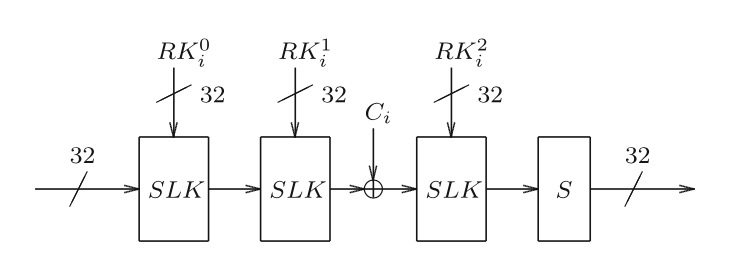
\includegraphics[scale=0.6]{project/images/1.jpg}

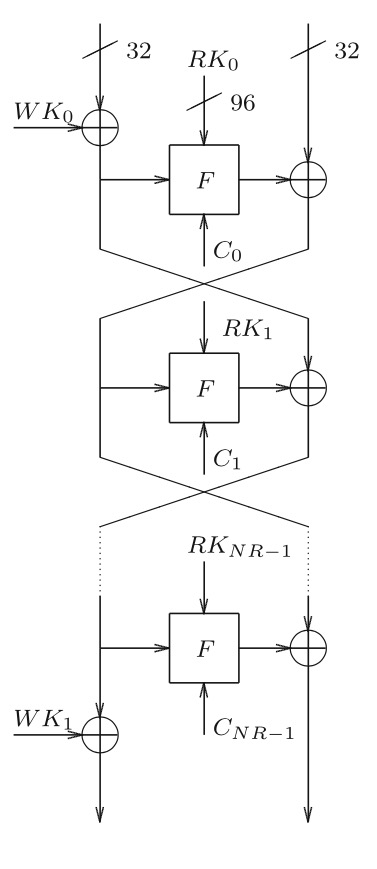
\includegraphics[scale=0.6]{project/images/2.jpg}

This is the  internal structure of the function F in figure 1 that is basically a SLK function that is the consecutive application of S-box layer(S) ,Diffusion Layer(L) and Key addition (K).


\section*{\fontsize{20}{24}\selectfont{\color{red} {Substitution and Diffusion:}}}

When X (figure 1) that is basically a 32 bit when going into F function then first it will go to the S -box which is basically the following:

{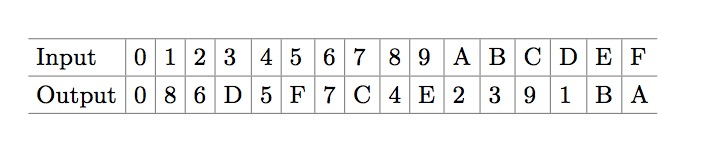
\includegraphics[scale=0.6]{project/images/4.jpg}}

Bit slice S-box structure has advantage in both hardware and software implementations. In software, the per- mutations before and after the S-boxes disappear. In hardware, on the other hand, they can be implemented by a simple wiring which consumes no extra area. 

The bits(permutation) gets substituted according to the S-box and a new permutation is formed after coming out from the S-box which is followed by the diffusion in the L box as follows:

After the bitslice S-box layer, we used a linear function on each byte of the state to provide diffusion inside 8-bit words. 

So we needed an efficient linear function operating on bytes. One classical solution for such a linear function for CPUs is using XOR of shifted and rotated values of the input word. 

We try to build linear functions of the form :


\includegraphics[scale=0.5]{project/images/5.jpg}

\section*{\fontsize{20}{24}\selectfont{\color{red} {Key Addition:}}}\\

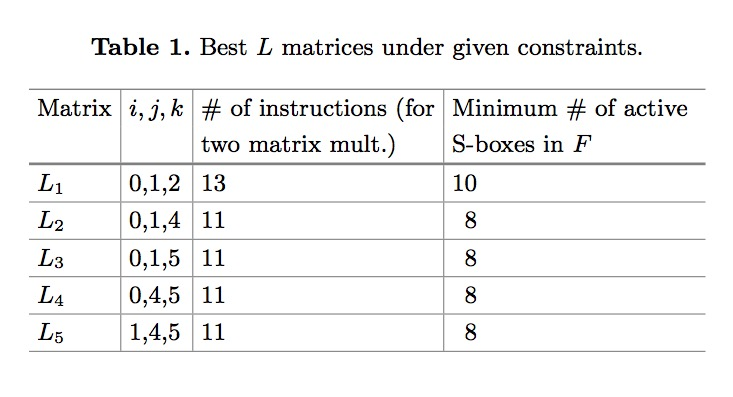
\includegraphics[scale=0.6]{project/images/6.jpg}

For example, if master key is 128-bit, it will be divided into 4 words of 32-bit as A∥B∥C∥D. Initial whitening key is A, first round key is B-C-D, second round key is A-B-C, etc. 

We call it as Whitening Key because its basic  function is to xor the initial bits in round 1 and the final bits after the last round.

\section*{\fontsize{20}{24}\selectfont{\color{red} {What Ci Represents?}}}\\

After the second SLK function, round constant is XORed to the least significant byte (rightmost byte, i.e., x3) of the state. For round i = 0,1,...,NR − 1, the round constant is Ci = NR − i, where NR is the number of rounds, and Ci is represented as 8-bit little endian integer, that is 12 = 00001100, 11 = 00001011, etc. 



\newpage% adds the Literature Survey page
\section*{\fontsize{25}{29}\selectfont{\textbf Contribution} \\}

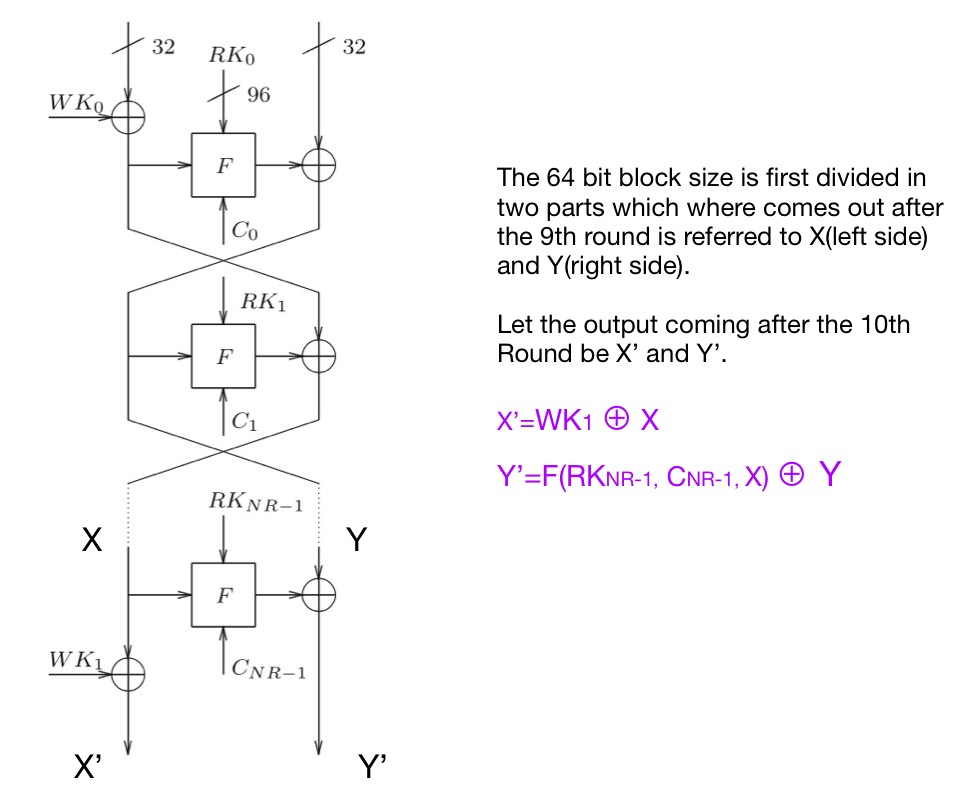
\includegraphics[scale=0.5]{project/images/7.jpg}

Now the equations 1 and 2 came when we have not induced any fault at any step.

Now let us put a fault after the 9th round such that Y becomes Y1.

Now the perceived output show some change and let the new output be Y1’.

Now the change in equation is :


\includegraphics[scale=0.5]{project/images/8.jpg}

Here the known variables are X’ ,Y’ and Y1’
and unknown variables are X,Y,X’,Y’,WK1
Now we are working on to solve 5 unknown variables and We are exploring the function F and we are also trying to reduce the  fair complexity in decrypting the function F. We have 3 equations and from this we will try to decipher the key using some mathematical operations on the equations.

Now we are doing Faults:\\

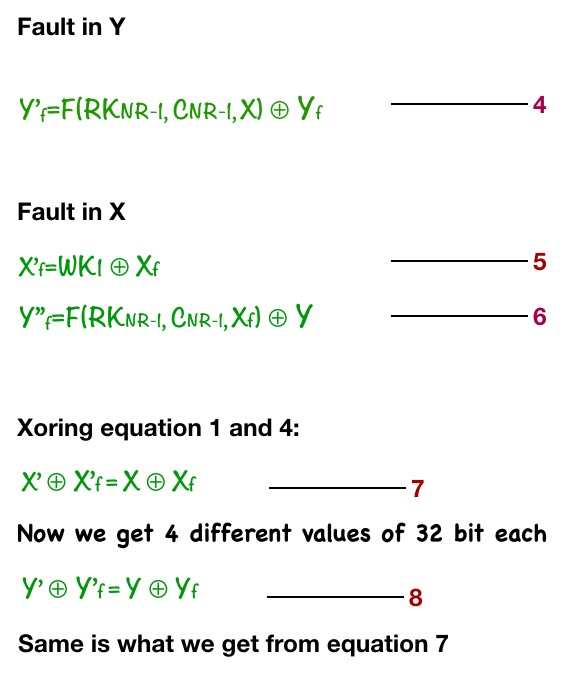
\includegraphics[scale=0.7]{project/images/9.jpg}

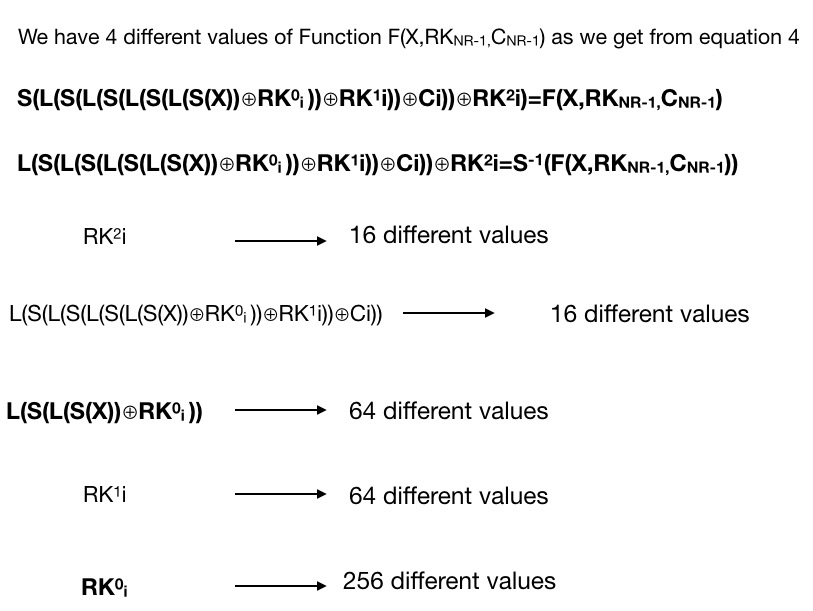
\includegraphics[scale=0.60]{project/images/10.jpg}


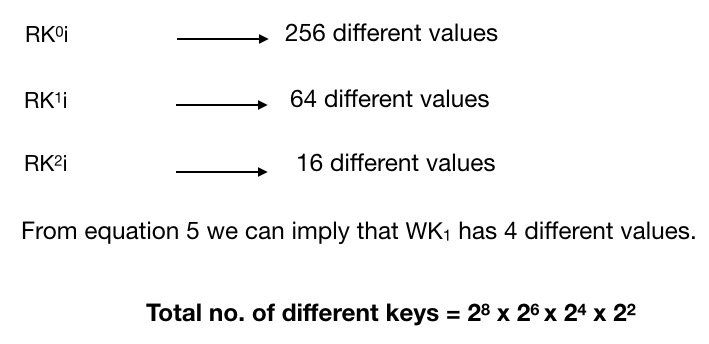
\includegraphics[scale=0.70]{project/images/11.jpg}

Now we reduce the exhaustive search space for possible keys of RoadRunneR:

\hspace{3.5cm}
\includegraphics[scale=0.60]{project/images/12.jpg}



\newpage
\section*{\fontsize{25}{29}\selectfont{\textbf Conclusion} \\}


A very efficient Feistel type bitslice block cipher, RoadRunneR, with 64-bit block size and 80-bit or 128-bit key length was presented. RoadRunneR is a perfect choice for devices with very restricted memory resources and for applications requiring reasonable throughput expectations. Our cipher has a high security margin in contrast to most of other lightweight block ciphers.\\

We did a fault attack on the block cipher and found the related equations. Then we derived an algorithm to find the solutions to those equations. We have proposed all the possibiliy of the pair of keys which could have been found.

 % adds the Scheduling and Planning page
\newpage
\section*{\fontsize{25}{29}\selectfont{\textbf Future Work} \\}

We have derived an algorithm to find the key by doing Fault attack on RoadRunneR and thus we are on the way of implementing a program which can find out the key of the block cipher when it receive a cipher text.

Additionally we have also initialized writing our first research paper providing a relevant and substantial thesis of the Fault attack we did on the block cipher.
\newpage
\section*{\fontsize{25}{29}\selectfont{\textbf References} \\}


1. Adnan Baysal and Sühap Şahin \\ TÜBİTAK BİLGEM, 41470 Gebze, Kocaeli, Turkey,
Department of Computer Engineering, Kocaeli University 41380 Umuttepe Yerleşkesi, Turkey
\\ {\color{blue}adnan.baysal@tubitak.gov.tr}\\ \\
2. Differential Fault Analysis of AES-128 Key Schedule using a Single Multi-Byte Fault \\
Sk Subidh Ali and Debdeep Mukhopadhyay (Dept. of Computer Science and Engineering
Indian Institute of Technology Kharagpur \\ India). \\ {\color{blue}debdeep@cse.iitkgp.ernet.in} \\ \\
3. Differential Fault Analysis of the Advanced Encryption Standard using a Single Fault \\ 
Michael Tunstall(Department of Computer Science, University of Bristol,Merchant Venturers Building \\ Woodland Road,Bristol BS8 1UB, United Kingdom. {\color{blue}@cs.bris.ac.uk)} \\ Debdeep Mukhopadhyay and Subidh Ali (Computer Sc. and Engg, IIT Kharagpur, India \\ {\color{blue}debdeep,subidh@cse.iitkgp.ernet.in)} \\
4. {\color{blue}https://www.youtube.com/watch?v=2aHkqB2-46k&t=28 }( Cryptography by Christof Paar) % adds the References page

\end{document}